\documentclass{article}\usepackage{graphicx, color}
%% maxwidth is the original width if it is less than linewidth
%% otherwise use linewidth (to make sure the graphics do not exceed the margin)
\makeatletter
\def\maxwidth{ %
  \ifdim\Gin@nat@width>\linewidth
    \linewidth
  \else
    \Gin@nat@width
  \fi
}
\makeatother

\IfFileExists{upquote.sty}{\usepackage{upquote}}{}
\definecolor{fgcolor}{rgb}{0.2, 0.2, 0.2}
\newcommand{\hlnumber}[1]{\textcolor[rgb]{0,0,0}{#1}}%
\newcommand{\hlfunctioncall}[1]{\textcolor[rgb]{0.501960784313725,0,0.329411764705882}{\textbf{#1}}}%
\newcommand{\hlstring}[1]{\textcolor[rgb]{0.6,0.6,1}{#1}}%
\newcommand{\hlkeyword}[1]{\textcolor[rgb]{0,0,0}{\textbf{#1}}}%
\newcommand{\hlargument}[1]{\textcolor[rgb]{0.690196078431373,0.250980392156863,0.0196078431372549}{#1}}%
\newcommand{\hlcomment}[1]{\textcolor[rgb]{0.180392156862745,0.6,0.341176470588235}{#1}}%
\newcommand{\hlroxygencomment}[1]{\textcolor[rgb]{0.43921568627451,0.47843137254902,0.701960784313725}{#1}}%
\newcommand{\hlformalargs}[1]{\textcolor[rgb]{0.690196078431373,0.250980392156863,0.0196078431372549}{#1}}%
\newcommand{\hleqformalargs}[1]{\textcolor[rgb]{0.690196078431373,0.250980392156863,0.0196078431372549}{#1}}%
\newcommand{\hlassignement}[1]{\textcolor[rgb]{0,0,0}{\textbf{#1}}}%
\newcommand{\hlpackage}[1]{\textcolor[rgb]{0.588235294117647,0.709803921568627,0.145098039215686}{#1}}%
\newcommand{\hlslot}[1]{\textit{#1}}%
\newcommand{\hlsymbol}[1]{\textcolor[rgb]{0,0,0}{#1}}%
\newcommand{\hlprompt}[1]{\textcolor[rgb]{0.2,0.2,0.2}{#1}}%

\usepackage{framed}
\makeatletter
\newenvironment{kframe}{%
 \def\at@end@of@kframe{}%
 \ifinner\ifhmode%
  \def\at@end@of@kframe{\end{minipage}}%
  \begin{minipage}{\columnwidth}%
 \fi\fi%
 \def\FrameCommand##1{\hskip\@totalleftmargin \hskip-\fboxsep
 \colorbox{shadecolor}{##1}\hskip-\fboxsep
     % There is no \\@totalrightmargin, so:
     \hskip-\linewidth \hskip-\@totalleftmargin \hskip\columnwidth}%
 \MakeFramed {\advance\hsize-\width
   \@totalleftmargin\z@ \linewidth\hsize
   \@setminipage}}%
 {\par\unskip\endMakeFramed%
 \at@end@of@kframe}
\makeatother

\definecolor{shadecolor}{rgb}{.97, .97, .97}
\definecolor{messagecolor}{rgb}{0, 0, 0}
\definecolor{warningcolor}{rgb}{1, 0, 1}
\definecolor{errorcolor}{rgb}{1, 0, 0}
\newenvironment{knitrout}{}{} % an empty environment to be redefined in TeX

\usepackage{alltt}

\title{STATS 209 - Take Home 2}
\author{Rene Kizilcec}
\date{March 8, 2013}
\usepackage[cm]{fullpage}

\begin{document}
\maketitle 




\begin{knitrout}
\definecolor{shadecolor}{rgb}{0.969, 0.969, 0.969}\color{fgcolor}\begin{kframe}
\begin{verbatim}
## 
##  MatchIt (Version 2.4-20, built: 2011-10-24)
##  Please refer to http://gking.harvard.edu/matchit for full documentation 
##  or help.matchit() for help with commands supported by MatchIt.
##
\end{verbatim}
\end{kframe}
\end{knitrout}


\section*{Problem 1}

\begin{knitrout}
\definecolor{shadecolor}{rgb}{0.969, 0.969, 0.969}\color{fgcolor}\begin{kframe}
\begin{alltt}
\hlfunctioncall{data}(Prestige)
Prestige=\hlfunctioncall{subset}(Prestige, !\hlfunctioncall{is.na}(type))
Prestige$type=\hlfunctioncall{ifelse}(Prestige$type==\hlstring{"bc"},\hlstring{"bc"},\hlstring{"pwc"})
\hlfunctioncall{table}(Prestige$type)
\end{alltt}
\begin{verbatim}

 bc pwc 
 44  54 
\end{verbatim}
\begin{alltt}
Prestige$type=\hlfunctioncall{as.numeric}(\hlfunctioncall{as.factor}(Prestige$type))-1
\end{alltt}
\end{kframe}
\end{knitrout}


\subsection*{part a}
\begin{knitrout}
\definecolor{shadecolor}{rgb}{0.969, 0.969, 0.969}\color{fgcolor}\begin{kframe}
\begin{alltt}
\hlfunctioncall{t.test}(prestige~type, Prestige, var.equal=T)
\end{alltt}
\begin{verbatim}

	Two Sample t-test

data:  prestige by type 
t = -7.872, df = 96, p-value = 5.309e-12
alternative hypothesis: true difference in means is not equal to 0 
95 percent confidence interval:
 -26.82 -16.01 
sample estimates:
mean in group 0 mean in group 1 
          35.53           56.94 

\end{verbatim}
\begin{alltt}
\hlfunctioncall{summary}(\hlfunctioncall{lm}(prestige~type+education, Prestige))
\end{alltt}
\begin{verbatim}

Call:
lm(formula = prestige ~ type + education, data = Prestige)

Residuals:
    Min      1Q  Median      3Q     Max 
-22.252  -5.683   0.898   5.719  16.334 

Coefficients:
            Estimate Std. Error t value Pr(>|t|)    
(Intercept)   -17.82       4.53   -3.94  0.00016 ***
type           -6.80       2.86   -2.38  0.01951 *  
education       6.38       0.52   12.27  < 2e-16 ***
---
Signif. codes:  0 '***' 0.001 '**' 0.01 '*' 0.05 '.' 0.1 ' ' 1 

Residual standard error: 8.38 on 95 degrees of freedom
Multiple R-squared: 0.765,	Adjusted R-squared: 0.76 
F-statistic:  154 on 2 and 95 DF,  p-value: <2e-16 

\end{verbatim}
\begin{alltt}
\hlfunctioncall{cor.test}(Prestige$type,Prestige$education)
\end{alltt}
\begin{verbatim}

	Pearson's product-moment correlation

data:  Prestige$type and Prestige$education 
t = 13.25, df = 96, p-value < 2.2e-16
alternative hypothesis: true correlation is not equal to 0 
95 percent confidence interval:
 0.7205 0.8645 
sample estimates:
  cor 
0.804 

\end{verbatim}
\end{kframe}
\end{knitrout}

Mean of BC group is 35.527 and mean of PWC is 56.943. The difference in means is 21.406 prestige points, which is highly significant according to our two sample t-test.

The ANCOVA computes a difference in means of -6.798 i.e. the main effect is now reversed: BC professions have more prestige when adding education as a covariate. The main effect is still significnat with p=0.02. The coefficient on Education is highly significantly different from zero and is positive, suggesting that more years of education are associated with greater prestige.

The problem is that the type variable and yrs. of education are highly correlated r=0.8, leading to a colinearity problem in the regression (or ANCOVA).

\subsection*{part b}
\begin{knitrout}
\definecolor{shadecolor}{rgb}{0.969, 0.969, 0.969}\color{fgcolor}\begin{kframe}
\begin{alltt}
m1=\hlfunctioncall{lm}(prestige~type+education, Prestige)
m2=\hlfunctioncall{lm}(prestige~type*education, Prestige)
\hlfunctioncall{anova}(m1,m2)
\end{alltt}
\begin{verbatim}
Analysis of Variance Table

Model 1: prestige ~ type + education
Model 2: prestige ~ type * education
  Res.Df  RSS Df Sum of Sq    F Pr(>F)  
1     95 6668                           
2     94 6471  1       197 2.87  0.094 .
---
Signif. codes:  0 '***' 0.001 '**' 0.01 '*' 0.05 '.' 0.1 ' ' 1 
\end{verbatim}
\begin{alltt}
\hlfunctioncall{summary}(m2)
\end{alltt}
\begin{verbatim}

Call:
lm(formula = prestige ~ type * education, data = Prestige)

Residuals:
    Min      1Q  Median      3Q     Max 
-19.709  -6.045   0.737   6.301  16.141 

Coefficients:
               Estimate Std. Error t value Pr(>|t|)    
(Intercept)       -4.29       9.17   -0.47    0.641    
type             -26.34      11.89   -2.22    0.029 *  
education          4.76       1.09    4.39    3e-05 ***
type:education     2.09       1.23    1.69    0.094 .  
---
Signif. codes:  0 '***' 0.001 '**' 0.01 '*' 0.05 '.' 0.1 ' ' 1 

Residual standard error: 8.3 on 94 degrees of freedom
Multiple R-squared: 0.772,	Adjusted R-squared: 0.764 
F-statistic:  106 on 3 and 94 DF,  p-value: <2e-16 

\end{verbatim}
\end{kframe}
\end{knitrout}

Comparing the previous model to the same model with a type:education interaction term added yields that the interaction is not significant at the 0.05 level. Closer inspection of the new model shows that the inclusion of the interaction term has increased the main effect of type, such that the mean difference at education=0 is 26.33. However, that is extrapolating, as nobody has zero education. What is interesting is that each additional year of education for workers in the PWC group is associated with 6.9 more prestige points, but only 4.8 points for workers in the BC group.

Anyway, but overall, as p-value adhering social scientists, we'd probably delete the interaction and stick to the two main effects.

\subsection*{part c}
\begin{knitrout}
\definecolor{shadecolor}{rgb}{0.969, 0.969, 0.969}\color{fgcolor}\begin{kframe}
\begin{alltt}
\hlfunctioncall{cbind}(\hlfunctioncall{c}(\hlstring{"BC"},\hlstring{"PWC"}),
    \hlfunctioncall{round}(\hlfunctioncall{predict}(m2,newdata=\hlfunctioncall{data.frame}(type=\hlfunctioncall{c}(0,1),education=\hlfunctioncall{c}(10,10)),interval=\hlstring{"conf"}),3))
\end{alltt}
\begin{verbatim}
        fit      lwr      upr     
1 "BC"  "43.343" "39.02"  "47.666"
2 "PWC" "37.894" "33.961" "41.827"
\end{verbatim}
\begin{alltt}
\hlfunctioncall{mean}(Prestige$education)
\end{alltt}
\begin{verbatim}
[1] 10.8
\end{verbatim}
\end{kframe}
\end{knitrout}

For 10yrs of educ. the ANCOVA model with interaction estimates 43.343 for BC and 37.894 for PWC, a -5.449 difference in means. However, the 95\% conf. intervals of the two estimates overlap, which means that the difference is in fact not significantly different from zero.
Looking at this for 10 years of education is interesting, because the average years of education in the sample is 10.8. Thus, we are not interpolating, but estimate data points that we actually have data on AND the T-Test above told us that the prestige means of the two groups are highly significantly different, but the ANCOVA tells us they're not.

\subsection*{part d}
\begin{knitrout}
\definecolor{shadecolor}{rgb}{0.969, 0.969, 0.969}\color{fgcolor}\begin{kframe}
\begin{alltt}
\hlcomment{# function to compute treatment effect \hlfunctioncall{alpha} (same as in handout)}
\hlcomment{# takes beta as input}
computeAlpha=\hlfunctioncall{function}(beta)\{
    Ydiff=\hlfunctioncall{with}(Prestige, \hlfunctioncall{mean}(prestige[type==1])-\hlfunctioncall{mean}(prestige[type==0]))
    Xdiff=\hlfunctioncall{with}(Prestige, \hlfunctioncall{mean}(education[type==1])-\hlfunctioncall{mean}(education[type==0]))
    \hlfunctioncall{return}(Ydiff-beta*Xdiff)    
\}
\hlfunctioncall{summary}(\hlfunctioncall{lm}(prestige~type, Prestige))
\end{alltt}
\begin{verbatim}

Call:
lm(formula = prestige ~ type, data = Prestige)

Residuals:
    Min      1Q  Median      3Q     Max 
-30.443  -9.793   0.515   9.607  30.257 

Coefficients:
            Estimate Std. Error t value Pr(>|t|)    
(Intercept)    35.53       2.02   17.59  < 2e-16 ***
type           21.42       2.72    7.87  5.3e-12 ***
---
Signif. codes:  0 '***' 0.001 '**' 0.01 '*' 0.05 '.' 0.1 ' ' 1 

Residual standard error: 13.4 on 96 degrees of freedom
Multiple R-squared: 0.392,	Adjusted R-squared: 0.386 
F-statistic:   62 on 1 and 96 DF,  p-value: 5.31e-12 

\end{verbatim}
\begin{alltt}
    \hlcomment{#coef should match beta=0}
\hlfunctioncall{summary}(\hlfunctioncall{lm}(prestige~type+education, Prestige))
\end{alltt}
\begin{verbatim}

Call:
lm(formula = prestige ~ type + education, data = Prestige)

Residuals:
    Min      1Q  Median      3Q     Max 
-22.252  -5.683   0.898   5.719  16.334 

Coefficients:
            Estimate Std. Error t value Pr(>|t|)    
(Intercept)   -17.82       4.53   -3.94  0.00016 ***
type           -6.80       2.86   -2.38  0.01951 *  
education       6.38       0.52   12.27  < 2e-16 ***
---
Signif. codes:  0 '***' 0.001 '**' 0.01 '*' 0.05 '.' 0.1 ' ' 1 

Residual standard error: 8.38 on 95 degrees of freedom
Multiple R-squared: 0.765,	Adjusted R-squared: 0.76 
F-statistic:  154 on 2 and 95 DF,  p-value: <2e-16 

\end{verbatim}
\begin{alltt}
    \hlcomment{#ANCOVA coef on X  = 6.3823}
\hlfunctioncall{summary}(\hlfunctioncall{lm}(prestige~type*education, Prestige))
\end{alltt}
\begin{verbatim}

Call:
lm(formula = prestige ~ type * education, data = Prestige)

Residuals:
    Min      1Q  Median      3Q     Max 
-19.709  -6.045   0.737   6.301  16.141 

Coefficients:
               Estimate Std. Error t value Pr(>|t|)    
(Intercept)       -4.29       9.17   -0.47    0.641    
type             -26.34      11.89   -2.22    0.029 *  
education          4.76       1.09    4.39    3e-05 ***
type:education     2.09       1.23    1.69    0.094 .  
---
Signif. codes:  0 '***' 0.001 '**' 0.01 '*' 0.05 '.' 0.1 ' ' 1 

Residual standard error: 8.3 on 94 degrees of freedom
Multiple R-squared: 0.772,	Adjusted R-squared: 0.764 
F-statistic:  106 on 3 and 94 DF,  p-value: <2e-16 

\end{verbatim}
\begin{alltt}
    \hlcomment{#control slope = 4.764}

\hlfunctioncall{computeAlpha}(0) \hlcomment{#t-test}
\end{alltt}
\begin{verbatim}
[1] 21.42
\end{verbatim}
\begin{alltt}
\hlfunctioncall{computeAlpha}(6.3823) \hlcomment{#standard ANCOVA}
\end{alltt}
\begin{verbatim}
[1] -6.798
\end{verbatim}
\begin{alltt}
betaYX.G=6.3823 \hlcomment{#from ancova above}
rYX.G=\hlfunctioncall{cor}(\hlfunctioncall{lm}(prestige~type,Prestige)$resid, \hlfunctioncall{lm}(education~type,Prestige)$resid)
\hlfunctioncall{computeAlpha}( betaYX.G/rYX.G ) \hlcomment{#Valididty Correction}
\end{alltt}
\begin{verbatim}
[1] -14.62
\end{verbatim}
\begin{alltt}
\hlfunctioncall{computeAlpha}(4.764) \hlcomment{#Belson}
\end{alltt}
\begin{verbatim}
[1] 0.3561
\end{verbatim}
\end{kframe}
\end{knitrout}

Method 1: 21.415 higher prestige for PWC compared to BC on average

Method 2: -6.7978 for educ=0; 5.449 lower prestige for PWC compared to BC given 10yrs of education (from part c)

Method 3: -14.621 prestige difference between PWC and BC; PWC has lower prestige than BC

Method 4: 0.3561 higher prestige for PWC compared to BC

\newpage
\section*{QUESTION 2}


\subsection*{part a}
\begin{knitrout}
\definecolor{shadecolor}{rgb}{0.969, 0.969, 0.969}\color{fgcolor}\begin{kframe}
\begin{alltt}
m1=\hlfunctioncall{lm}(wage~education, PSID1982)
\hlcomment{#\hlfunctioncall{summary}(m1)}
\hlfunctioncall{cbind}(coef=\hlfunctioncall{coef}(m1),\hlfunctioncall{confint}(m1))
\end{alltt}
\begin{verbatim}
             coef   2.5 % 97.5 %
(Intercept) 70.47 -110.67 251.61
education   83.89   70.11  97.67
\end{verbatim}
\end{kframe}
\end{knitrout}

The presumed increase in wage for each additional year of education is 84  with 95\% CI = (70, 98). 

It is very likely for there to be omitted variables like skills, intelligence, work experience to name but a few. The estimated coefficient on education in this simple-minded regression is biased as a result of leaving out these variables in the regression. 
We cannot make an "as if by experiment" conclusion because years of education is not randomly assigned but instead depends on many things that we do not observe (and that are not in the regression model). Thus, people differ in other variables in systematic ways that are confounded with years of education.

\subsection*{part b}
\begin{knitrout}
\definecolor{shadecolor}{rgb}{0.969, 0.969, 0.969}\color{fgcolor}\begin{kframe}
\begin{alltt}
PSID1982$industry=\hlfunctioncall{as.numeric}(PSID1982$industry)-1
\hlfunctioncall{cor.test}(~industry+education, PSID1982)
\end{alltt}
\begin{verbatim}

	Pearson's product-moment correlation

data:  industry and education 
t = -6.228, df = 593, p-value = 8.977e-10
alternative hypothesis: true correlation is not equal to 0 
95 percent confidence interval:
 -0.3217 -0.1708 
sample estimates:
    cor 
-0.2478 

\end{verbatim}
\begin{alltt}
\hlfunctioncall{cor.test}(~industry+wage, PSID1982)
\end{alltt}
\begin{verbatim}

	Pearson's product-moment correlation

data:  industry and wage 
t = 0.6565, df = 593, p-value = 0.5118
alternative hypothesis: true correlation is not equal to 0 
95 percent confidence interval:
 -0.05355  0.10710 
sample estimates:
    cor 
0.02695 

\end{verbatim}
\end{kframe}
\end{knitrout}

As promised, moderate significant correlation with education and tiny insignificant correlation with wage. This satisfies the basic IV requirements for an instrument (just the basic ones: we don't know about things we don't know about ...). From this we would hope that the only way 'industry' is associated with wage is through education. From the regression above, we have reason to believe that education and wage are strongly associated.

\begin{knitrout}
\definecolor{shadecolor}{rgb}{0.969, 0.969, 0.969}\color{fgcolor}\begin{kframe}
\begin{alltt}
\hlfunctioncall{summary}(\hlfunctioncall{ivreg}(wage~education|industry,data=PSID1982))
\end{alltt}
\begin{verbatim}

Call:
ivreg(formula = wage ~ education | industry, data = PSID1982)

Residuals:
   Min     1Q Median     3Q    Max 
-956.4 -366.2  -74.1  219.6 4038.0 

Coefficients:
            Estimate Std. Error t value Pr(>|t|)    
(Intercept)   1414.0      427.1    3.31  0.00099 ***
education      -20.7       33.2   -0.62  0.53319    
---
Signif. codes:  0 '***' 0.001 '**' 0.01 '*' 0.05 '.' 0.1 ' ' 1 

Residual standard error: 559 on 593 degrees of freedom
Multiple R-Squared: -0.108,	Adjusted R-squared: -0.11 
Wald test: 0.389 on 1 and 593 DF,  p-value: 0.533 

\end{verbatim}
\end{kframe}
\end{knitrout}

Using industry as an instrument, it looks like there are no significant returns to education (good I'm not getting this PhD for a higher salary).
\begin{knitrout}
\definecolor{shadecolor}{rgb}{0.969, 0.969, 0.969}\color{fgcolor}\begin{kframe}
\begin{alltt}
Xhat=\hlfunctioncall{fitted}(\hlfunctioncall{lm}(education~industry,PSID1982)) \hlcomment{#step 1}
\hlfunctioncall{summary}(\hlfunctioncall{lm}(wage~Xhat,PSID1982)) \hlcomment{#step 2}
\end{alltt}
\begin{verbatim}

Call:
lm(formula = wage ~ Xhat, data = PSID1982)

Residuals:
   Min     1Q Median     3Q    Max 
  -844   -350    -66    207   3964 

Coefficients:
            Estimate Std. Error t value Pr(>|t|)    
(Intercept)   1414.0      405.7    3.49  0.00053 ***
Xhat           -20.7       31.5   -0.66  0.51178    
---
Signif. codes:  0 '***' 0.001 '**' 0.01 '*' 0.05 '.' 0.1 ' ' 1 

Residual standard error: 531 on 593 degrees of freedom
Multiple R-squared: 0.000726,	Adjusted R-squared: -0.000959 
F-statistic: 0.431 on 1 and 593 DF,  p-value: 0.512 

\end{verbatim}
\begin{alltt}
\hlfunctioncall{with}(PSID1982, \hlfunctioncall{cov}(wage,industry)/\hlfunctioncall{cov}(education,industry)) \hlcomment{#slopes}
\end{alltt}
\begin{verbatim}
[1] -20.7
\end{verbatim}
\end{kframe}
\end{knitrout}

Coefficients are the same for all, but std. error higher in IV and TSLS compared to OLS. This shows that if only a weak instrument is available, accepting some bias may be better than increasing variance due to the weakness of the instrument.

\subsection*{part c}
\begin{knitrout}
\definecolor{shadecolor}{rgb}{0.969, 0.969, 0.969}\color{fgcolor}\begin{kframe}
\begin{alltt}
PSID1982=\hlfunctioncall{subset}(PSID1982, gender==\hlstring{"male"})

m1=\hlfunctioncall{lm}(wage~education, PSID1982)
\hlfunctioncall{cbind}(coef=\hlfunctioncall{coef}(m1),\hlfunctioncall{confint}(m1))
\end{alltt}
\begin{verbatim}
              coef  2.5 % 97.5 %
(Intercept) 111.35 -78.46  301.2
education    84.77  70.34   99.2
\end{verbatim}
\begin{alltt}

\hlfunctioncall{cor.test}(~industry+education, PSID1982)
\end{alltt}
\begin{verbatim}

	Pearson's product-moment correlation

data:  industry and education 
t = -6.266, df = 526, p-value = 7.701e-10
alternative hypothesis: true correlation is not equal to 0 
95 percent confidence interval:
 -0.3412 -0.1823 
sample estimates:
    cor 
-0.2636 

\end{verbatim}
\begin{alltt}
\hlfunctioncall{cor.test}(~industry+wage, PSID1982)
\end{alltt}
\begin{verbatim}

	Pearson's product-moment correlation

data:  industry and wage 
t = -0.5815, df = 526, p-value = 0.5611
alternative hypothesis: true correlation is not equal to 0 
95 percent confidence interval:
 -0.11044  0.06011 
sample estimates:
     cor 
-0.02535 

\end{verbatim}
\begin{alltt}

\hlfunctioncall{summary}(\hlfunctioncall{ivreg}(wage~education|industry,data=PSID1982))
\end{alltt}
\begin{verbatim}

Call:
ivreg(formula = wage ~ education | industry, data = PSID1982)

Residuals:
   Min     1Q Median     3Q    Max 
-872.0 -326.2  -57.5  182.9 3824.3 

Coefficients:
            Estimate Std. Error t value Pr(>|t|)  
(Intercept)    967.3      385.7    2.51    0.012 *
education       18.1       30.0    0.61    0.545  
---
Signif. codes:  0 '***' 0.001 '**' 0.01 '*' 0.05 '.' 0.1 ' ' 1 

Residual standard error: 512 on 526 degrees of freedom
Multiple R-Squared: 0.0772,	Adjusted R-squared: 0.0754 
Wald test: 0.366 on 1 and 526 DF,  p-value: 0.545 

\end{verbatim}
\begin{alltt}
Xhat=\hlfunctioncall{fitted}(\hlfunctioncall{lm}(education~industry,PSID1982)) \hlcomment{#step 1}
\hlfunctioncall{summary}(\hlfunctioncall{lm}(wage~Xhat,PSID1982)) \hlcomment{#step 2}
\end{alltt}
\begin{verbatim}

Call:
lm(formula = wage ~ Xhat, data = PSID1982)

Residuals:
   Min     1Q Median     3Q    Max 
  -920   -335    -80    215   3888 

Coefficients:
            Estimate Std. Error t value Pr(>|t|)  
(Intercept)    967.3      401.4    2.41    0.016 *
Xhat            18.1       31.2    0.58    0.561  
---
Signif. codes:  0 '***' 0.001 '**' 0.01 '*' 0.05 '.' 0.1 ' ' 1 

Residual standard error: 533 on 526 degrees of freedom
Multiple R-squared: 0.000642,	Adjusted R-squared: -0.00126 
F-statistic: 0.338 on 1 and 526 DF,  p-value: 0.561 

\end{verbatim}
\begin{alltt}
\hlfunctioncall{with}(PSID1982, \hlfunctioncall{cov}(wage,industry)/\hlfunctioncall{cov}(education,industry)) \hlcomment{#slopes}
\end{alltt}
\begin{verbatim}
[1] 18.14
\end{verbatim}
\end{kframe}
\end{knitrout}

Now, just looking at males. I'd expect it to not make much difference given that there were many more males than females in the sample.

Simple-minded: 85 with 95\% CI = (70, 99); almost the same.

Correlations: basic requirements of instrument 'industry' still hold.
education     -20.70      33.21  -0.624 0.533190    

IVREG, TSLS, Slopes: Coefficient on education not significant, using instrument.

All in all, it is the same thing, as expected.

\subsection*{part d}
Diff in mortality for Trt-Ctrl = (18.2-19.4)/100 = -.012
Diff in compliance Trt-Ctrl = 708/1065-1813/2695 = -0.008
IV est = -.012/-.008 = 1.5

\subsection*{part e}
The following values are percentage point differences, so that we can easily check for significance using the provided SE intervals.

Intent-to-Treat (ITT): 18.2-19.4 = -1.2 (not significant)

As-Treated Analysis: 15-(24.6*257 + 19.4*2695)/(257+2695) = -4.853 (maybe sig.)

Per-Protocol Analysis: 15-19.4 = -4.4 (SEs don't overlap, maybe sig.)

CACE (Complier Average Causal Effect): 15-15.1 = -0.1 (not significant)

ITT and CACE are not significant. The effect lies in whether people comply or not. This is picked up by As-Treated and Per-Protocol, though it is incorrectly attributed to the effectiveness of the drug.

\newpage
\section*{QUESTION 3}
\begin{knitrout}
\definecolor{shadecolor}{rgb}{0.969, 0.969, 0.969}\color{fgcolor}\begin{kframe}
\begin{alltt}
\hlfunctioncall{data}(\hlstring{"Guns"})
Guns=\hlfunctioncall{subset}(Guns, year == 1999)
\end{alltt}
\end{kframe}
\end{knitrout}

\subsection*{part a}
\begin{knitrout}
\definecolor{shadecolor}{rgb}{0.969, 0.969, 0.969}\color{fgcolor}\begin{kframe}
\begin{alltt}
\hlfunctioncall{par}(mfrow=\hlfunctioncall{c}(1,2))
\hlfunctioncall{boxplot}(violent~law, Guns,main=\hlstring{"Violent"})
\hlfunctioncall{boxplot}(\hlfunctioncall{log}(violent)~law, Guns,main=\hlstring{"\hlfunctioncall{log}(Violent)"})
\end{alltt}
\end{kframe}

{\centering 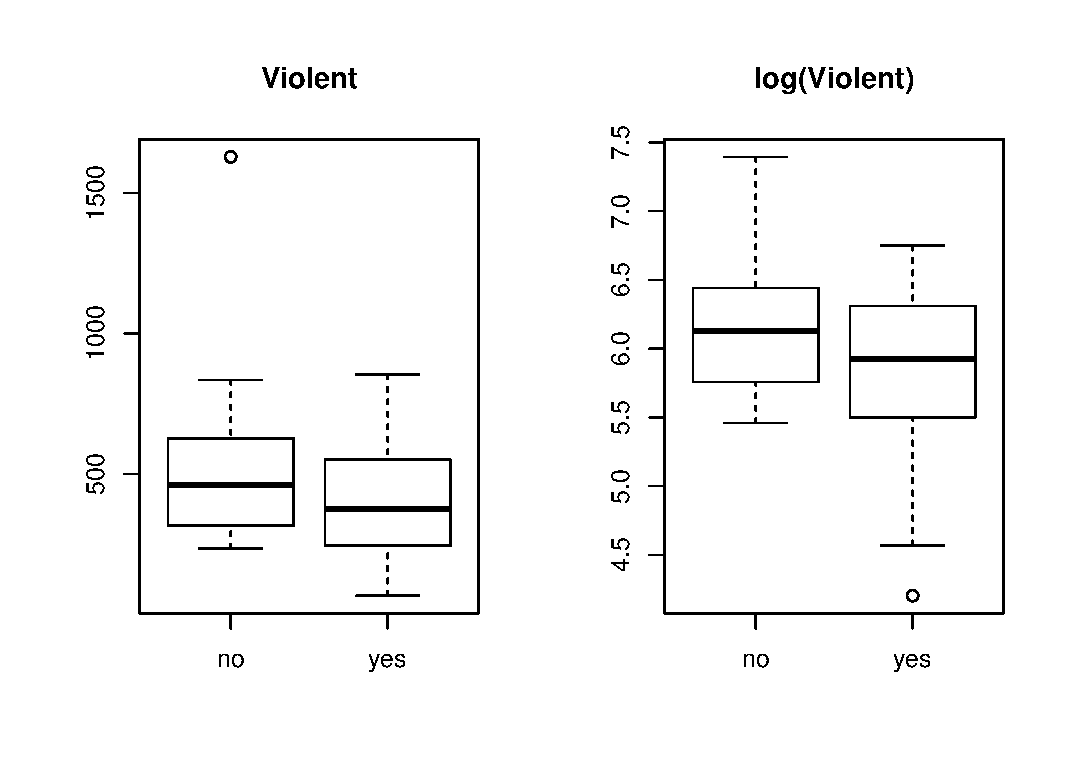
\includegraphics[width=\linewidth]{plots/unnamed-chunk-14} 

}


\end{knitrout}

\begin{knitrout}
\definecolor{shadecolor}{rgb}{0.969, 0.969, 0.969}\color{fgcolor}\begin{kframe}
\begin{alltt}
\hlfunctioncall{par}(mfrow=\hlfunctioncall{c}(1,2))
\hlfunctioncall{hist}(Guns$violent)
\hlfunctioncall{hist}(\hlfunctioncall{log}(Guns$violent))
\end{alltt}
\end{kframe}

{\centering 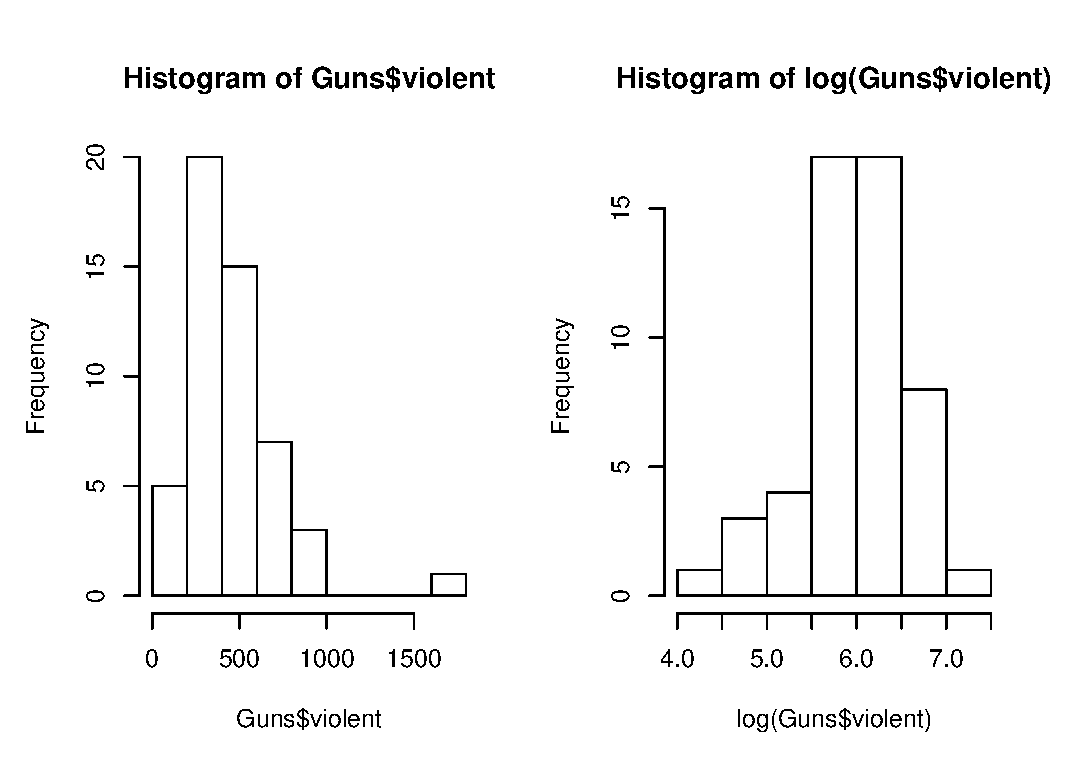
\includegraphics[width=\linewidth]{plots/unnamed-chunk-15} 

}


\end{knitrout}

\begin{knitrout}
\definecolor{shadecolor}{rgb}{0.969, 0.969, 0.969}\color{fgcolor}\begin{kframe}
\begin{alltt}
\hlfunctioncall{table}(Guns$law)
\end{alltt}
\begin{verbatim}

 no yes 
 22  29 
\end{verbatim}
\begin{alltt}
\hlfunctioncall{fivenum}(Guns[Guns$law==\hlstring{"no"},]$violent)
\end{alltt}
\begin{verbatim}
[1]  235.0  316.4  460.2  627.2 1627.7
\end{verbatim}
\begin{alltt}
\hlfunctioncall{fivenum}(Guns[Guns$law==\hlstring{"yes"},]$violent)
\end{alltt}
\begin{verbatim}
[1]  66.9 244.9 374.9 551.2 854.0
\end{verbatim}
\begin{alltt}
\hlfunctioncall{fivenum}(\hlfunctioncall{log}(Guns[Guns$law==\hlstring{"no"},]$violent))
\end{alltt}
\begin{verbatim}
[1] 5.460 5.757 6.130 6.441 7.395
\end{verbatim}
\begin{alltt}
\hlfunctioncall{fivenum}(\hlfunctioncall{log}(Guns[Guns$law==\hlstring{"yes"},]$violent))
\end{alltt}
\begin{verbatim}
[1] 4.203 5.501 5.927 6.312 6.750
\end{verbatim}
\begin{alltt}
\hlfunctioncall{ddply}(Guns, \hlfunctioncall{.}(law), summarize, mean=\hlfunctioncall{mean}(violent), sd=\hlfunctioncall{sd}(violent),
      logMean=\hlfunctioncall{mean}(\hlfunctioncall{log}(violent)), logSd=\hlfunctioncall{sd}(\hlfunctioncall{log}(violent)))
\end{alltt}
\begin{verbatim}
  law  mean    sd logMean  logSd
1  no 525.1 305.4   6.144 0.4785
2 yes 407.9 218.3   5.833 0.6641
\end{verbatim}
\begin{alltt}
\hlfunctioncall{t.test}(violent~law, Guns)
\end{alltt}
\begin{verbatim}

	Welch Two Sample t-test

data:  violent by law 
t = 1.528, df = 36.34, p-value = 0.1351
alternative hypothesis: true difference in means is not equal to 0 
95 percent confidence interval:
 -38.3 272.8 
sample estimates:
 mean in group no mean in group yes 
            525.1             407.9 

\end{verbatim}
\begin{alltt}
\hlfunctioncall{t.test}(\hlfunctioncall{log}(violent)~law, Guns)
\end{alltt}
\begin{verbatim}

	Welch Two Sample t-test

data:  log(violent) by law 
t = 1.937, df = 48.9, p-value = 0.05849
alternative hypothesis: true difference in means is not equal to 0 
95 percent confidence interval:
 -0.01157  0.63174 
sample estimates:
 mean in group no mean in group yes 
            6.144             5.833 

\end{verbatim}
\end{kframe}
\end{knitrout}


I used Welch two sample t-tests, because we have reason to believe that variances are not equal between groups.

The log transformation helps make the distribution of violent more normal, as can be seen from the histograms above. This is necessary to use a t-test that relies on certain distributional assumptions.

The t-test on the logged violent data suggests that groups are different and we know that the mean violence in states where law=no is higher. This suggests: more guns, less crime. BUT we don't actually know if people have MORE guns. So rather: allow guns, less crime. Moreover, there is confounding because laws aren't randomly assigned.

\subsection*{part b}
\begin{knitrout}
\definecolor{shadecolor}{rgb}{0.969, 0.969, 0.969}\color{fgcolor}\begin{kframe}
\begin{alltt}
\hlfunctioncall{t.test}(\hlfunctioncall{log}(income)~law, Guns)
\end{alltt}
\begin{verbatim}

	Welch Two Sample t-test

data:  log(income) by law 
t = 3.96, df = 37.69, p-value = 0.0003212
alternative hypothesis: true difference in means is not equal to 0 
95 percent confidence interval:
 0.07586 0.23466 
sample estimates:
 mean in group no mean in group yes 
            9.784             9.629 

\end{verbatim}
\end{kframe}
\end{knitrout}

We log income, as economists tend to do, and see that the groups of states differ significantly in average income.
\begin{knitrout}
\definecolor{shadecolor}{rgb}{0.969, 0.969, 0.969}\color{fgcolor}\begin{kframe}
\begin{alltt}
Guns$prop=\hlfunctioncall{glm}(law~prisoners+afam+cauc+male+population+income+density, 
    Guns, family=\hlfunctioncall{binomial}())$fitted
\hlfunctioncall{sortFrame}(Guns,prop)[\hlfunctioncall{c}(1,51),\hlfunctioncall{c}(12:14)]
\end{alltt}
\begin{verbatim}
                   state law      prop
207 District of Columbia  no 6.495e-09
621              Montana yes 9.434e-01
\end{verbatim}
\end{kframe}
\end{knitrout}

Lowest for DC, highest for Montana. 
\begin{knitrout}
\definecolor{shadecolor}{rgb}{0.969, 0.969, 0.969}\color{fgcolor}\begin{kframe}
\begin{alltt}
\hlfunctioncall{par}(mfrow=\hlfunctioncall{c}(1,1))
\hlfunctioncall{boxplot}(prop~law, Guns)
\end{alltt}
\end{kframe}

{\centering 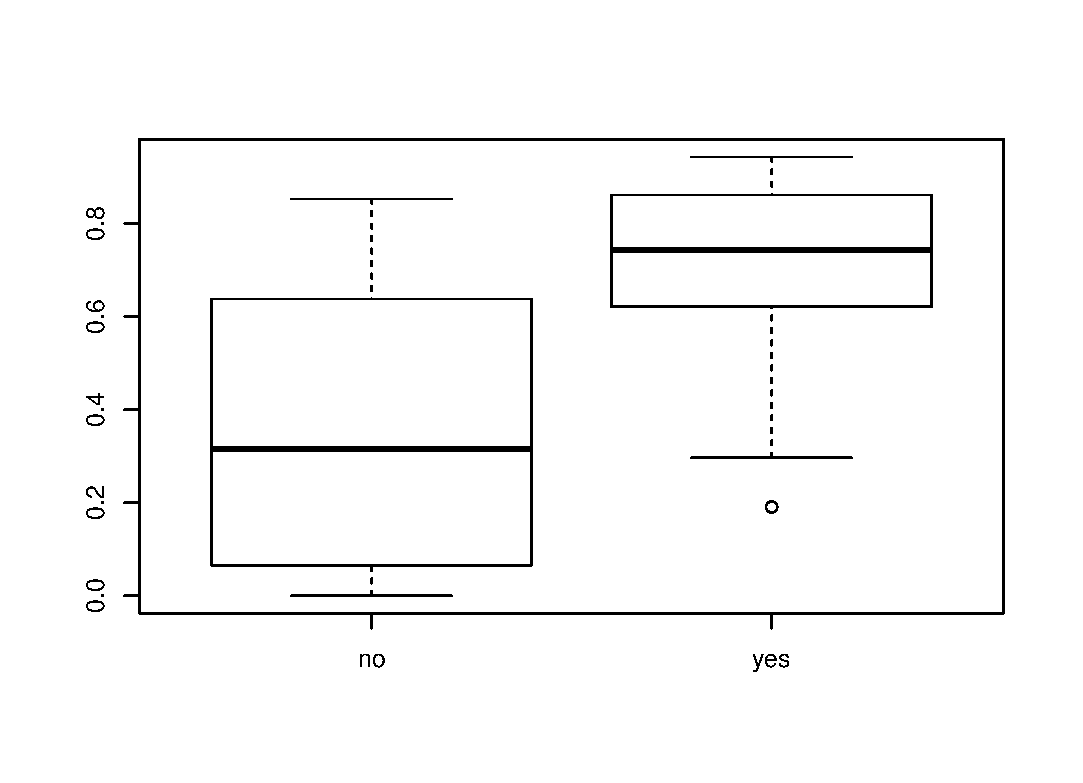
\includegraphics[width=\linewidth]{plots/unnamed-chunk-19} 

}


\end{knitrout}

Distribution of propensity shows some overlap of the quartiles.

\subsection*{part c}
Given that we only have 51 data points (22 in one group, 29 in the other), it is unlikely that subclassification in 5 groups is feasible. There would be too few observations (states) in the subclasses.
\begin{knitrout}
\definecolor{shadecolor}{rgb}{0.969, 0.969, 0.969}\color{fgcolor}\begin{kframe}
\begin{alltt}
cutoffs=\hlfunctioncall{quantile}(Guns$prop, probs=\hlfunctioncall{seq}(0,1,1/3))
Guns$prop3=NA
Guns[Guns$prop<cutoffs[2],]$prop3=0
Guns[Guns$prop<cutoffs[3] & Guns$prop>=cutoffs[2],]$prop3=1
Guns[Guns$prop>=cutoffs[3],]$prop3=2
\hlfunctioncall{ddply}(Guns, \hlfunctioncall{.}(law,prop3), summarize, meanProp=\hlfunctioncall{mean}(prop))
\end{alltt}
\begin{verbatim}
  law prop3 meanProp
1  no     0   0.1266
2  no     1   0.6264
3  no     2   0.8382
4 yes     0   0.3831
5 yes     1   0.6576
6 yes     2   0.8639
\end{verbatim}
\begin{alltt}
\hlfunctioncall{ddply}(Guns, \hlfunctioncall{.}(law,prop3), summarize, meanIncome=\hlfunctioncall{mean}(income), meanPris=\hlfunctioncall{mean}(prisoners))
\end{alltt}
\begin{verbatim}
  law prop3 meanIncome meanPris
1  no     0      19711    472.5
2  no     1      16440    353.6
3  no     2      13398    395.0
4 yes     0      17689    315.6
5 yes     1      15741    372.1
6 yes     2      14224    400.9
\end{verbatim}
\end{kframe}
\end{knitrout}

Across law, the balance of the propensities within each (of the three) propensity groups is ok for medium and high propensity, but not very balanced for the low propensity group (.13 for 'no' vs. .38 for 'yes'). 
Comparing the balance of income and prisoners for law yes vs. no states within strata yields that the low propensity strata is less balanced than the other two.
\begin{knitrout}
\definecolor{shadecolor}{rgb}{0.969, 0.969, 0.969}\color{fgcolor}\begin{kframe}
\begin{alltt}
\hlcomment{#\hlfunctioncall{t.test}(violent~law, Guns, subset=prop3==0)}
\hlcomment{#\hlfunctioncall{t.test}(violent~law, Guns, subset=prop3==1)}
\hlcomment{#\hlfunctioncall{t.test}(violent~law, Guns, subset=prop3==2)}
\hlfunctioncall{t.test}(\hlfunctioncall{log}(violent)~law, Guns, subset=prop3==0)
\end{alltt}
\begin{verbatim}

	Welch Two Sample t-test

data:  log(violent) by law 
t = 1.123, df = 5.7, p-value = 0.3064
alternative hypothesis: true difference in means is not equal to 0 
95 percent confidence interval:
 -0.5249  1.3948 
sample estimates:
 mean in group no mean in group yes 
            6.244             5.809 

\end{verbatim}
\begin{alltt}
\hlfunctioncall{t.test}(\hlfunctioncall{log}(violent)~law, Guns, subset=prop3==1)
\end{alltt}
\begin{verbatim}

	Welch Two Sample t-test

data:  log(violent) by law 
t = -0.7062, df = 13.82, p-value = 0.4918
alternative hypothesis: true difference in means is not equal to 0 
95 percent confidence interval:
 -0.5151  0.2601 
sample estimates:
 mean in group no mean in group yes 
            5.914             6.041 

\end{verbatim}
\begin{alltt}
\hlfunctioncall{t.test}(\hlfunctioncall{log}(violent)~law, Guns, subset=prop3==2)
\end{alltt}
\begin{verbatim}

	Welch Two Sample t-test

data:  log(violent) by law 
t = 2.271, df = 2.255, p-value = 0.1367
alternative hypothesis: true difference in means is not equal to 0 
95 percent confidence interval:
 -0.5231  2.0105 
sample estimates:
 mean in group no mean in group yes 
            6.461             5.717 

\end{verbatim}
\end{kframe}
\end{knitrout}

Two sample t-tests within each strata now indicate no significant difference between states with law=yes and law=no. (Neither with violent, nor log(violent))
I'm somewhat reliefed.

\subsection*{part d}

\begin{knitrout}
\definecolor{shadecolor}{rgb}{0.969, 0.969, 0.969}\color{fgcolor}\begin{kframe}
\begin{alltt}
m1=\hlfunctioncall{matchit}(\hlfunctioncall{I}(\hlfunctioncall{as.numeric}(law)-1)~prisoners+afam+cauc+male+population+income+density, 
           data=Guns, method=\hlstring{"full"})
m1
\end{alltt}
\begin{verbatim}

Call: 
matchit(formula = I(as.numeric(law) - 1) ~ prisoners + afam + 
    cauc + male + population + income + density, data = Guns, 
    method = "full")

Sample sizes:
          Control Treated
All            22      29
Matched        22      29
Unmatched       0       0
Discarded       0       0

\end{verbatim}
\begin{alltt}
\hlfunctioncall{ddply}(\hlfunctioncall{match.data}(m1), \hlfunctioncall{.}(subclass), summarize, violent=\hlfunctioncall{mean}(violent), logViolent=\hlfunctioncall{mean}(\hlfunctioncall{log}(violent)))
\end{alltt}
\begin{verbatim}
   subclass violent logViolent
1         1   374.0      5.743
2         2   310.2      5.715
3         3   612.9      6.389
4         4   487.1      6.152
5         5   437.6      5.840
6         6   308.0      5.725
7         7   185.2      5.091
8         8   416.1      6.011
9         9   523.9      6.241
10       10   223.7      5.378
11       11   646.4      6.330
12       12   458.4      6.114
\end{verbatim}
\begin{alltt}
\hlfunctioncall{ggplot}(\hlfunctioncall{match.data}(m1), \hlfunctioncall{aes}(law,\hlfunctioncall{log}(violent)))+\hlfunctioncall{geom_boxplot}()+\hlfunctioncall{facet_wrap}(~subclass)+\hlfunctioncall{theme_bw}()
\end{alltt}
\end{kframe}

{\centering 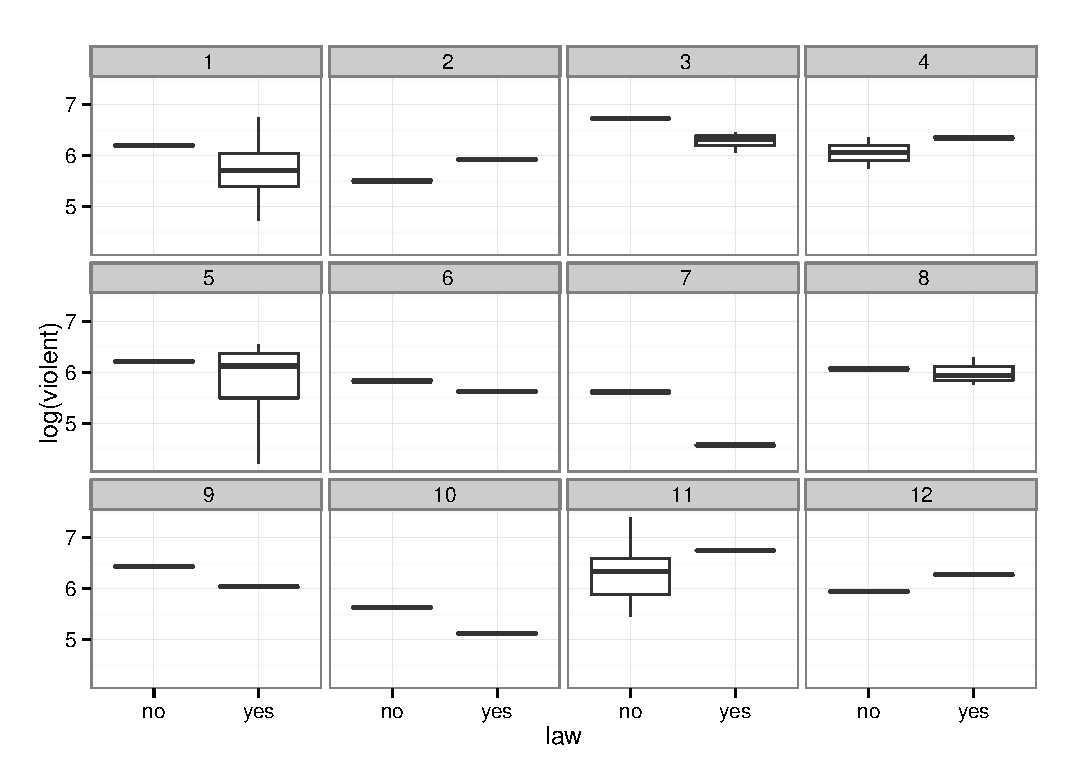
\includegraphics[width=\linewidth]{plots/unnamed-chunk-22} 

}


\end{knitrout}


Looking at the outcome meas for the 12 subclassifications (and the pretty plot) I looks like for most of them the means of violece are very similar, and more importantly, for some of them violence with lawYes is higher while for others violence with lawNo is higher. That means that once we start comparing statates that (in the ideal case) only differ in whether they are lawYes or lawNo, the aggregate group differences (probably caused by self-selection) are gone.

\end{document}
